\documentclass[a4paper]{article}

\usepackage[english]{babel}
\usepackage[utf8]{inputenc}
\usepackage{amsmath}
\usepackage{graphicx}
\usepackage[colorinlistoftodos]{todonotes}
\usepackage[left=2cm, right=2cm, top=2cm]{geometry} 
\usepackage{float}
\title{$S_N$ Method}

%\author{Your names and group number}

\date{\today}

\begin{document}
\maketitle



%\begin{figure}[H]
%\centering
%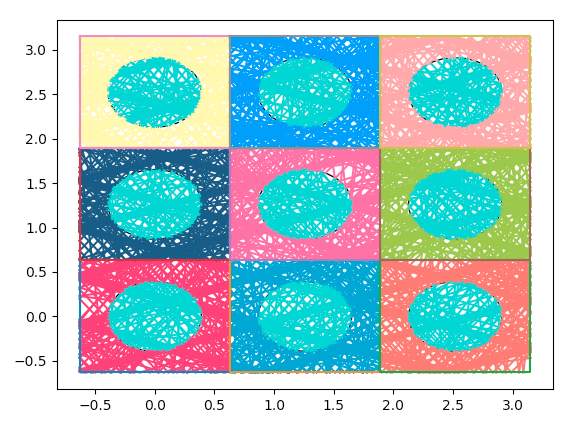
\includegraphics[width=0.8\textwidth]{raysPic}
%  \caption{\label{fig:fig1}} Here is a picture of my pincell 3x3 with a lot of rays in it.
%\end{figure}
The main equation that we want to solve is 
\[\mu_{n}\left(\psi_{i+\frac{1}{2},n}-\psi_{i-\frac{1}{2},n}\right)+\Delta_{i}\Sigma_{ti}\psi_{i,n}=\Delta_{i}Q_{i}\]
where $i$ is for the cell number, and $n$ is for $S_n$, and deals with the Gauss-Legendre quadrature order that we want to use. Like, for $S_2$ commonly $\mu_1=-\mu_2$ and $w_1=w_2=1$. 
 
 There are three approaches that we're going to use that start from here. Step, Diamond-Difference, and Step-Characteristics.
 \subsection*{Step}
 The main approximation here is that $\psi_i\approx\psi_{i-1/2}$ for $\mu>0$ and $\psi_i\approx\psi_{i+1/2}$ for $\mu<0$.
 \subsubsection*{$\mu>0$}
 \[\psi_i=\psi_{i-1/2}\]
\[\mu_n\left(\psi_{i+\frac{1}{2},n}-\psi_{i-\frac{1}{2},n}\right)+\Delta_i\Sigma_{ti}\psi_{i,n}=\Delta_iQ_i\]
\[\mu_n\left(\psi_{i+\frac{1}{2},n}-\psi_{i-\frac{1}{2},n}\right)+\Delta_i\Sigma_{ti}\psi_{i-1/2,n}=\Delta_iQ_i\]
And since we're traveling from left to right, that means we're starting with $i-1/2$ and we're trying to get to $i+1/2$. So I'll solve for $i+1/2$ in terms of $i-1/2$.
\[\psi_{i+\frac{1}{2},n}-\psi_{i-\frac{1}{2},n}=\frac{\Delta_iQ_i-\Delta_i\Sigma_{ti}\psi_{i-1/2,n}}{\mu_n}\]
\[\psi_{i+\frac{1}{2},n}=\frac{\Delta_iQ_i-\Delta_i\Sigma_{ti}\psi_{i-1/2,n}}{\mu_n}+\psi_{i-\frac{1}{2},n}\]
\[\boxed{\psi_{i+\frac{1}{2},n}=\frac{\Delta_iQ_i}{\mu_n}+\psi_{i-1/2,n}\left(1-\frac{\Delta_i\Sigma_{ti}}{\mu_n}\right)}\]


 \subsubsection*{$\mu<0$}
 \[\psi_i=\psi_{i+1/2}\]
\[\mu_n\left(\psi_{i+\frac{1}{2},n}-\psi_{i-\frac{1}{2},n}\right)+\Delta_i\Sigma_{ti}\psi_{i,n}=\Delta_iQ_i\]
\[\mu_n\left(\psi_{i+\frac{1}{2},n}-\psi_{i-\frac{1}{2},n}\right)+\Delta_i\Sigma_{ti}\psi_{i+1/2,n}=\Delta_iQ_i\]
And since we're traveling from right to left, that means we're starting with $i+1/2$ and we're trying to get to $i-1/2$. So I'll solve for $i-1/2$ in terms of $i+1/2$.
\[\psi_{i+\frac{1}{2},n}-\psi_{i-\frac{1}{2},n}=\frac{\Delta_iQ_i-\Delta_i\Sigma_{ti}\psi_{i+1/2,n}}{\mu_n}\]
%\[\psi_{i+\frac{1}{2},n}-\frac{\Delta_iQ_i-\Delta_i\Sigma_{ti}\psi_{i+1/2,n}}{\mu_n}=\psi_{i-\frac{1}{2},n}\]
\[\psi_{i-\frac{1}{2},n}=\psi_{i+\frac{1}{2},n}-\frac{\Delta_iQ_i-\Delta_i\Sigma_{ti}\psi_{i+1/2,n}}{\mu_n}\]
\[\boxed{\psi_{i-\frac{1}{2},n}=-\frac{\Delta_iQ_i}{\mu_n}+\psi_{i+\frac{1}{2},n}\left(1+\frac{\Delta_i\Sigma_{ti}}{\mu_n}\right)}\]





 \subsection*{Diamond-Difference}
 The main approximation here is that 
 \[\psi_{i,n}=\frac{\psi_{i-1/2,n}+\psi_{i+1/2,n}}{2}\]

 \subsubsection*{$\mu>0$}
\[\mu_n\left(\psi_{i+\frac{1}{2},n}-\psi_{i-\frac{1}{2},n}\right)+\Delta_i\Sigma_{ti}\psi_{i,n}=\Delta_iQ_i\]
\[\mu_n\left(\psi_{i+\frac{1}{2},n}-\psi_{i-\frac{1}{2},n}\right)+\Delta_i\Sigma_{ti}\frac{\psi_{i-1/2,n}+\psi_{i+1/2,n}}{2}=\Delta_iQ_i\]
And since we're traveling from left to right, that means we're starting with $i-1/2$ and we're trying to get to $i+1/2$. So I'll solve for $i+1/2$ in terms of $i-1/2$.
\[2\mu_n\psi_{i+\frac{1}{2},n}-2\mu_n\psi_{i-\frac{1}{2},n}+\Delta_i\Sigma_{ti}\psi_{i-1/2,n}+\Delta_i\Sigma_{ti}\psi_{i+1/2,n}=2\Delta_iQ_i\]
\[(\Delta_i\Sigma_{ti}+2\mu_n)\psi_{i+\frac{1}{2},n}+(\Delta_i\Sigma_{ti}-2\mu_n)\psi_{i-1/2,n}=2\Delta_iQ_i\]
\[\psi_{i+\frac{1}{2},n}=\frac{2\Delta_iQ_i-(\Delta_i\Sigma_{ti}-2\mu_n)\psi_{i-1/2,n}}{\Delta_i\Sigma_{ti}+2\mu_n}\]
\[\boxed{\psi_{i+\frac{1}{2},n}=\frac{2\mu_n-\Delta_i\Sigma_{ti}}{2\mu_n+\Delta_i\Sigma_{ti}}\psi_{i-1/2,n}+\frac{2\Delta_iQ_i}{\Delta_i\Sigma_{ti}+2\mu_n}}\]


 \subsubsection*{$\mu<0$}
\[\mu_n\left(\psi_{i+\frac{1}{2},n}-\psi_{i-\frac{1}{2},n}\right)+\Delta_i\Sigma_{ti}\psi_{i,n}=\Delta_iQ_i\]
\[\mu_n\left(\psi_{i+\frac{1}{2},n}-\psi_{i-\frac{1}{2},n}\right)+\Delta_i\Sigma_{ti}\frac{\psi_{i-1/2,n}+\psi_{i+1/2,n}}{2}=\Delta_iQ_i\]
And since we're traveling from right to left, that means we're starting with $i+1/2$ and we're trying to get to $i-1/2$. So I'll solve for $i-1/2$ in terms of $i+1/2$.
\[2\mu_n\psi_{i+\frac{1}{2},n}-2\mu_n\psi_{i-\frac{1}{2},n}+\Delta_i\Sigma_{ti}\psi_{i-1/2,n}+\Delta_i\Sigma_{ti}\psi_{i+1/2,n}=2\Delta_iQ_i\]
\[(\Delta_i\Sigma_{ti}+2\mu_n)\psi_{i+\frac{1}{2},n}+(\Delta_i\Sigma_{ti}-2\mu_n)\psi_{i-1/2,n}=2\Delta_iQ_i\]
\[(\Delta_i\Sigma_{ti}-2\mu_n)\psi_{i-1/2,n}=-(\Delta_i\Sigma_{ti}+2\mu_n)\psi_{i+\frac{1}{2},n}+2\Delta_iQ_i\]
\[\psi_{i-1/2,n}=\frac{-(\Delta_i\Sigma_{ti}+2\mu_n)}{(\Delta_i\Sigma_{ti}-2\mu_n)}\psi_{i+\frac{1}{2},n}+\frac{2\Delta_iQ_i}{(\Delta_i\Sigma_{ti}-2\mu_n)}\]
\[\boxed{\psi_{i-1/2,n}=\frac{2\mu_n+\Delta_i\Sigma_{ti}}{2\mu_n-\Delta_i\Sigma_{ti}}\psi_{i+\frac{1}{2},n}-\frac{2\Delta_iQ_i}{2\mu_n-\Delta_i\Sigma_{ti}}}\]





 \subsection*{Step-Characteristic}
 The main approximation here is that 
 \[\psi_{i,n}=\psi_{i-1/2,n}e^{-\Sigma_{ti}\Delta_i/\mu_n}+\frac{Q_i}{\Sigma_{ti}}\left(1-e^{-\Sigma_{ti}\Delta_i/\mu_n}\right)~\mbox{for }\mu>0\]
% \[\psi_{i,n}=\psi_{i+1/2,n}e^{-\Sigma_{ti}\Delta_i/\mu_n}+\frac{Q_i}{\Sigma_{ti}}\left(1-e^{-\Sigma_{ti}\Delta_i/\mu_n}\right)~\mbox{for }\mu>0\]

 \subsubsection*{$\mu>0$}
\[\mu_n\left(\psi_{i+\frac{1}{2},n}-\psi_{i-\frac{1}{2},n}\right)+\Delta_i\Sigma_{ti}\psi_{i,n}=\Delta_iQ_i\]
\[\mu_n\left(\psi_{i+\frac{1}{2},n}-\psi_{i-\frac{1}{2},n}\right)+\Delta_i\Sigma_{ti}\left(\psi_{i-1/2,n}e^{-\Sigma_{ti}\Delta_i/\mu_n}+\frac{Q_i}{\Sigma_{ti}}\left(1-e^{-\Sigma_{ti}\Delta_i/\mu_n}\right)\right)=\Delta_iQ_i\]
\[\mu_n\psi_{i+\frac{1}{2},n}-\mu_n\psi_{i-\frac{1}{2},n}+\Delta_i\Sigma_{ti}\psi_{i-1/2,n}e^{-\Sigma_{ti}\Delta_i/\mu_n}+\Delta_iQ_i-\Delta_iQ_ie^{-\Sigma_{ti}\Delta_i/\mu_n}=\Delta_iQ_i\]
And since we're traveling from left to right, that means we're starting with $i-1/2$ and we're trying to get to $i+1/2$. So I'll solve for $i+1/2$ in terms of $i-1/2$.
\[\mu_n\psi_{i+\frac{1}{2},n}=\Delta_iQ_i+\mu_n\psi_{i-\frac{1}{2},n}-\Delta_i\Sigma_{ti}\psi_{i-1/2,n}e^{-\Sigma_{ti}\Delta_i/\mu_n}-\Delta_iQ_i+\Delta_iQ_ie^{-\Sigma_{ti}\Delta_i/\mu_n}\]
\[\psi_{i+\frac{1}{2},n}=\psi_{i-\frac{1}{2},n}-\frac{\Delta_i\Sigma_{ti}}{\mu_n}\psi_{i-1/2,n}e^{-\Sigma_{ti}\Delta_i/\mu_n}+\frac{\Delta_iQ_i}{\mu_n}e^{-\Sigma_{ti}\Delta_i/\mu_n}\]
\[\boxed{\psi_{i+\frac{1}{2},n}=\left(1-\frac{\Delta_i\Sigma_{ti}}{\mu_n}e^{-\Sigma_{ti}\Delta_i/\mu_n}\right)\psi_{i-1/2,n}+\frac{\Delta_iQ_i}{\mu_n}e^{-\Sigma_{ti}\Delta_i/\mu_n}}\]

 %\subsubsection*{$\mu<0$}
%nd since we're traveling from right to left, that means we're starting with $i+1/2$ and we're trying to get to $i-1/2$. So I'll solve for $i-1/2$ in terms of $i+1/2$.



 \subsection*{Linear Discontinuous}
 So the idea of Linear Discontinuous is that we alternate between ``known'' values, and artificial values that make solving this problem easier. So when I'm going from left to right, I start with a known source at $i=1/2$. I use that to calculate an artificial value at $i=1/2$. This artificial value gives me the real value at $i=3/2$, which I then use to get the artificial values at $i=3/2$, etc.
 
 \subsubsection*{$\mu>0$}
 \[\mbox{Real}\quad\rightarrow\quad\mbox{Fake}\quad\rightarrow\quad\mbox{Real}\quad\rightarrow\quad\mbox{Fake}\quad\rightarrow\quad\mbox{Real}\quad\rightarrow\quad\mbox{Fake}\quad\rightarrow\quad\mbox{Real}\]
 \[\psi^R_{0}\quad\rightarrow\quad\psi^L_1\quad\rightarrow\quad\psi^R_1\quad\rightarrow\quad\psi^L_2\quad\rightarrow\quad\psi^R_2\quad\rightarrow\quad\psi^L_3\quad\rightarrow\quad\psi^R_3\]
where $\psi_0^R$ is the flux on the right side of the zero'th cell (or, in this indexing, the furthest left cell), and similarly, $\psi_3^R$ is the real flux on the right side of the third cell (which here is the furthest right cell).
\begin{enumerate}
  \item Compute source
  \item Solve for $\psi_{i,m}^L$ knowing $\psi_{i-1,m}^R$
    \[\psi_{i,m}^L=\frac{\left(\tilde{Q}^L+2\mu_m\psi_{i-1,m}^R-\Sigma_{t}\Delta x_{i}\frac{\tilde{Q}^R}{3T_{2/3}}-\mu_m\frac{\tilde{Q}^R}{T_{2/3}}\right)}{\left(\mu_m+\mu_m\frac{s_{1/3}}{T_{2/3}}+\frac{2\Sigma_{t}\Delta x_{i}}{3}+\frac{\Sigma_{t}\Delta x_{i}S_{1/3}}{3T_{2/3}}\right)}\]
    \[\tilde{Q}^{L}=\left(\frac{1}{3}Q^{R}+\frac{2}{3}Q^{L}\right)\Delta x\]
    \[\tilde{Q}^{R}=\left(\frac{2}{3}Q^{R}+\frac{1}{3}Q^{L}\right)\Delta x\]
  \item Solve for $\psi_{i,m}^R$ knowing $\psi_{i,m}^L$
    \[\psi_{i,m}^R=\frac{\tilde{Q}^R+\psi_{i,m}^{L}\left(\mu_{m}-\Sigma_{t,i}\Delta x_{i}/3\right)}{\left(\mu_{m}+2\Sigma_{t,i}\Delta x_{i}/3\right)}\]
    \[\tilde{Q}^{R}=\left(\frac{2}{3}Q^{R}+\frac{1}{3}Q^{L}\right)\Delta x\]

  \item Sweep form left to right
\end{enumerate}
\end{document}
